%
% problemstellung.tex -- Beispiel-File für die Beschreibung des Problems
%
% (c) 2020 Prof Dr Andreas Müller, Hochschule Rapperswil
%
\section{Beispiele von verwandten Funktionen
\label{logistic:section:beispiele}}
\rhead{Beispiele von verwandten Funktionen}
\begin{figure}[h!]
    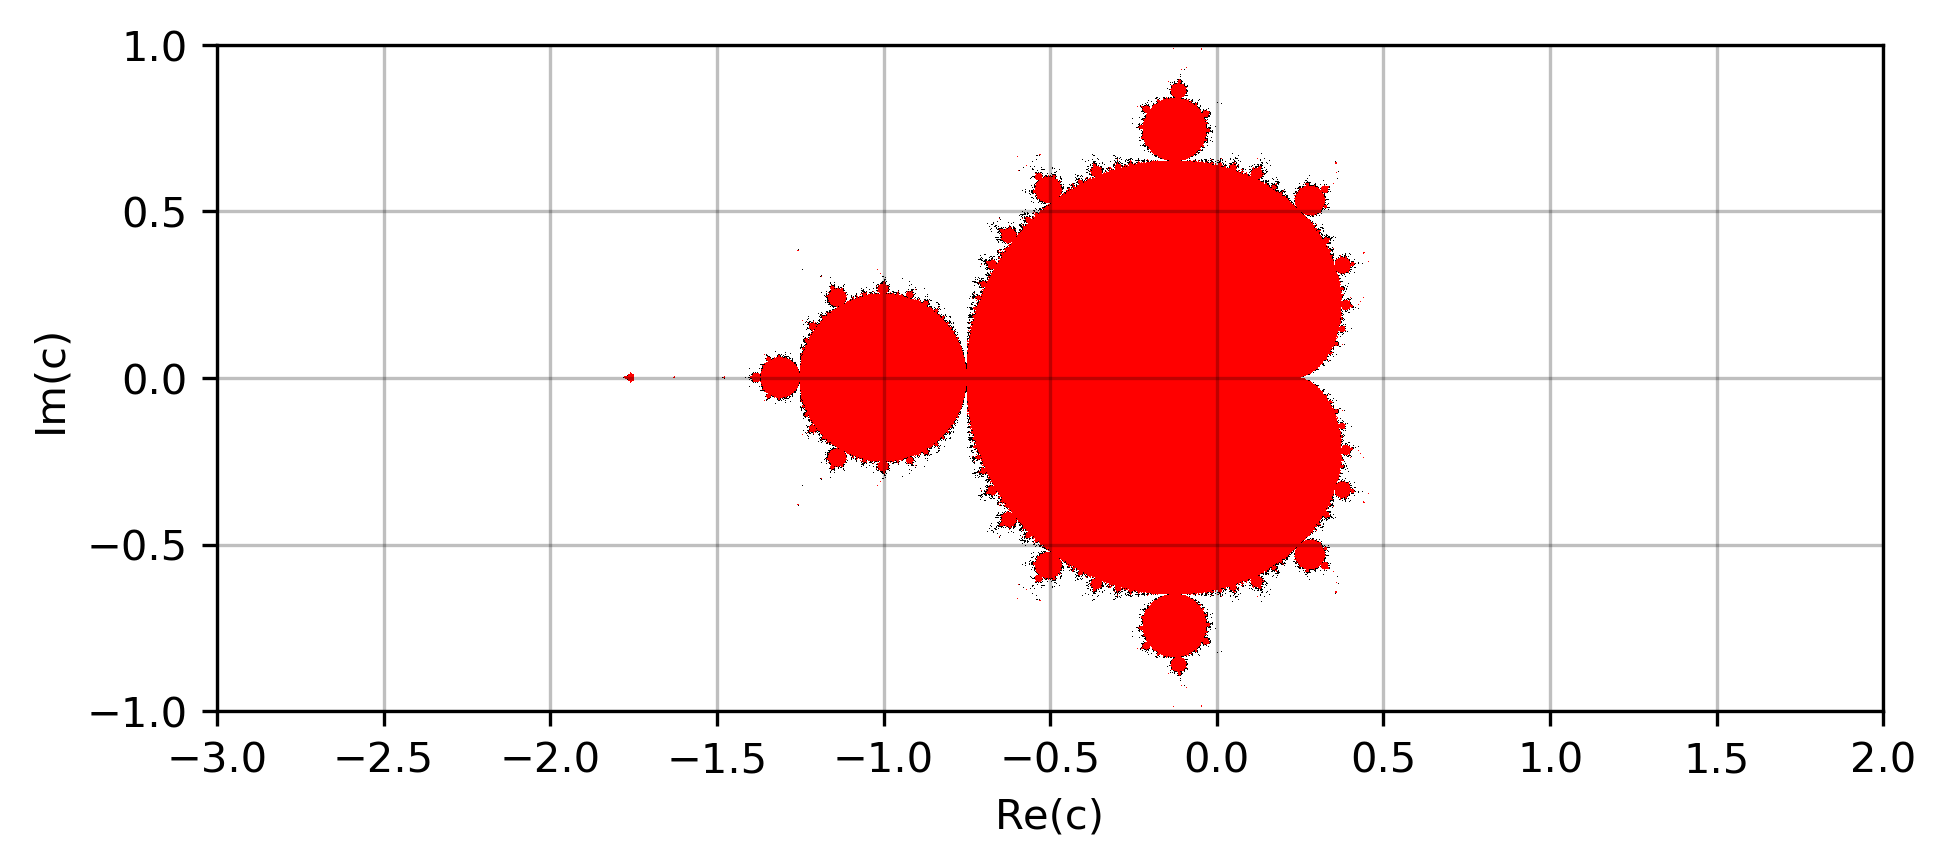
\includegraphics[width=\linewidth]{papers/logistic/figures/mandel.png}
    \caption{Mandelbrotmenge}
    \label{fig:mandel_2d}
\end{figure}
%\FloatBarrier
\subsection{Mandelbrotmenge}
\index{Mandelbrotmenge}%
\begin{figure}
    
\includegraphics[width=\linewidth]{papers/logistic/figures/mandel_3d.png}
    \caption{
        Dreidimensionales Bifurkationsdiagramm der Mandelbrotmenge.
        Das Bild wird aus einem flachen Winkel 
        leicht von oben angeschaut. 
        Die horizontale Ebene repräsentiert die
        Werte von $c$, siehe Abbildung \ref{fig:mandel_2d}
        zum Vergleich.
        Die vertikale Achse zeigt
        die Werte, die $\Re(z_n)$ annimmt wenn 
        $n \rightarrow \infty$.
        Rote Farbe bedeutet, dass $\Re(z_n)$ eine
        endliche Periode hat, schwarze Farbe bedeutet
        chaotisches Verhalten. 
        Besonders interessant ist das Gebilde auf der 
        linken Seite, das dem Bifurkationsdiagramm
        der logistischen Gleichung sehr änhlich sieht.
    }
    \label{fig:mandel_3d}
\end{figure}
In Kapitel \ref{logistic:section:analyse} 
haben wir bereits gesehen, 
dass das Bifurkationsdiagramm der logistischen Gleichung
ein Fraktal ist. 
Eines der bekanntesten Fraktale ist die Mandelbrotmenge,
deren Gleichung der logistischen Gleichung sehr ähnlich ist. 
Die Iterationsgleichung der Mandelbrotmenge lautet
\begin{equation}
    z_{n+1} = z_n^2 + c\text{,}
    \label{eq:mandelbrot}
\end{equation}
wobei $z_n$ und $c$ komplexe Zahlen sind und 
der Einfachkeit halber $z_0 = 0$ gesetzt werden kann.
Zum Vergleich, die logistische Gleichung hat ausmultipliziert
die Form $x_{n+1} = -\lambda x_n^2 +\lambda x_n$. 
Wie bei der logistischen Gleichung gibt es auch
bei der Gleichung der Mandelbrotmenge wieder bestimmte
Werte von $c$, bei der $z_n$ entweder 
divergiert, 
konvergiert, 
oszilliert 
oder in chaotisches Verhalten ausbricht. 
Jeder Wert von $c$, für den $z_n$ nicht 
divergiert, ist Teil der Mandelbrotmenge. 
Nun können wir, ähnlich wie schon beim 
Bifurkationsdiagramm der logistischen Gleichung, auf der
komplexen Ebene für jeden Wert von $c$ das Verhalten
der Gleichung der Mandelbrotmenge darstellen. 
Dazu färben wir den Bereich, in dem $z_n$ 
nicht divergiert, rot ein.
Damit sehen wir in Abbildung \ref{fig:mandel_2d}
die Mandelbrotmenge. 
Auf dieser zweidimensionalen Darstellung ist jedoch nicht zu sehen, 
welche Werte $z_n$ annimmt.
Darum nehmen wir jetzt die dritte Dimension zur Hilfe um,
wie schon beim Bifurkationsdiagramm der logistischen Gleichung,
auf der vertikalen Achse darzustellen, 
auf welchem Wert sich der Wert von $z_n$ schlussendlich einpendelt.
Oder eben auch nicht, wenn es oszilliert oder sogar
chaotisch wird. 
Da wir nur drei Dimensionen zur Verfügung haben,
beschränken uns dabei auf den Realteil von $z_n$. 
Das Ergebnis davon ist in Abbildung 
\ref{fig:mandel_3d}
zu sehen. 
Die Farben geben Auskunft über die Periodizität des 
jeweiligen Punktes. 
Rote Farbe bedeutet, dass $\Re(z_n)$
für den jeweiligen Wert von $c$ eine endliche 
Periode hat. 
Schwarz bedeutet chaotisches Verhalten 
oder möglicherweise auch,
dass die Periode so gross ist, dass der Computer
sie bei der Berechnung nicht als endlich erkannt hat.
Auf der reellen Achse ist deutlich ein Gebilde zu sehen,
welches dem Bifurkationsdiagramm der logistischen
Gleichung sehr ähnlich sieht. 
Ebenfalls zu sehen ist, dass die kreisförmigen
``Platformen'' sich regelmässig verdoppeln, weil
$\Re(z_n)$ zwischen immer mehr Werten hin und her oszilliert.

\subsection{Universelle Eigenschaft}
\begin{figure}
    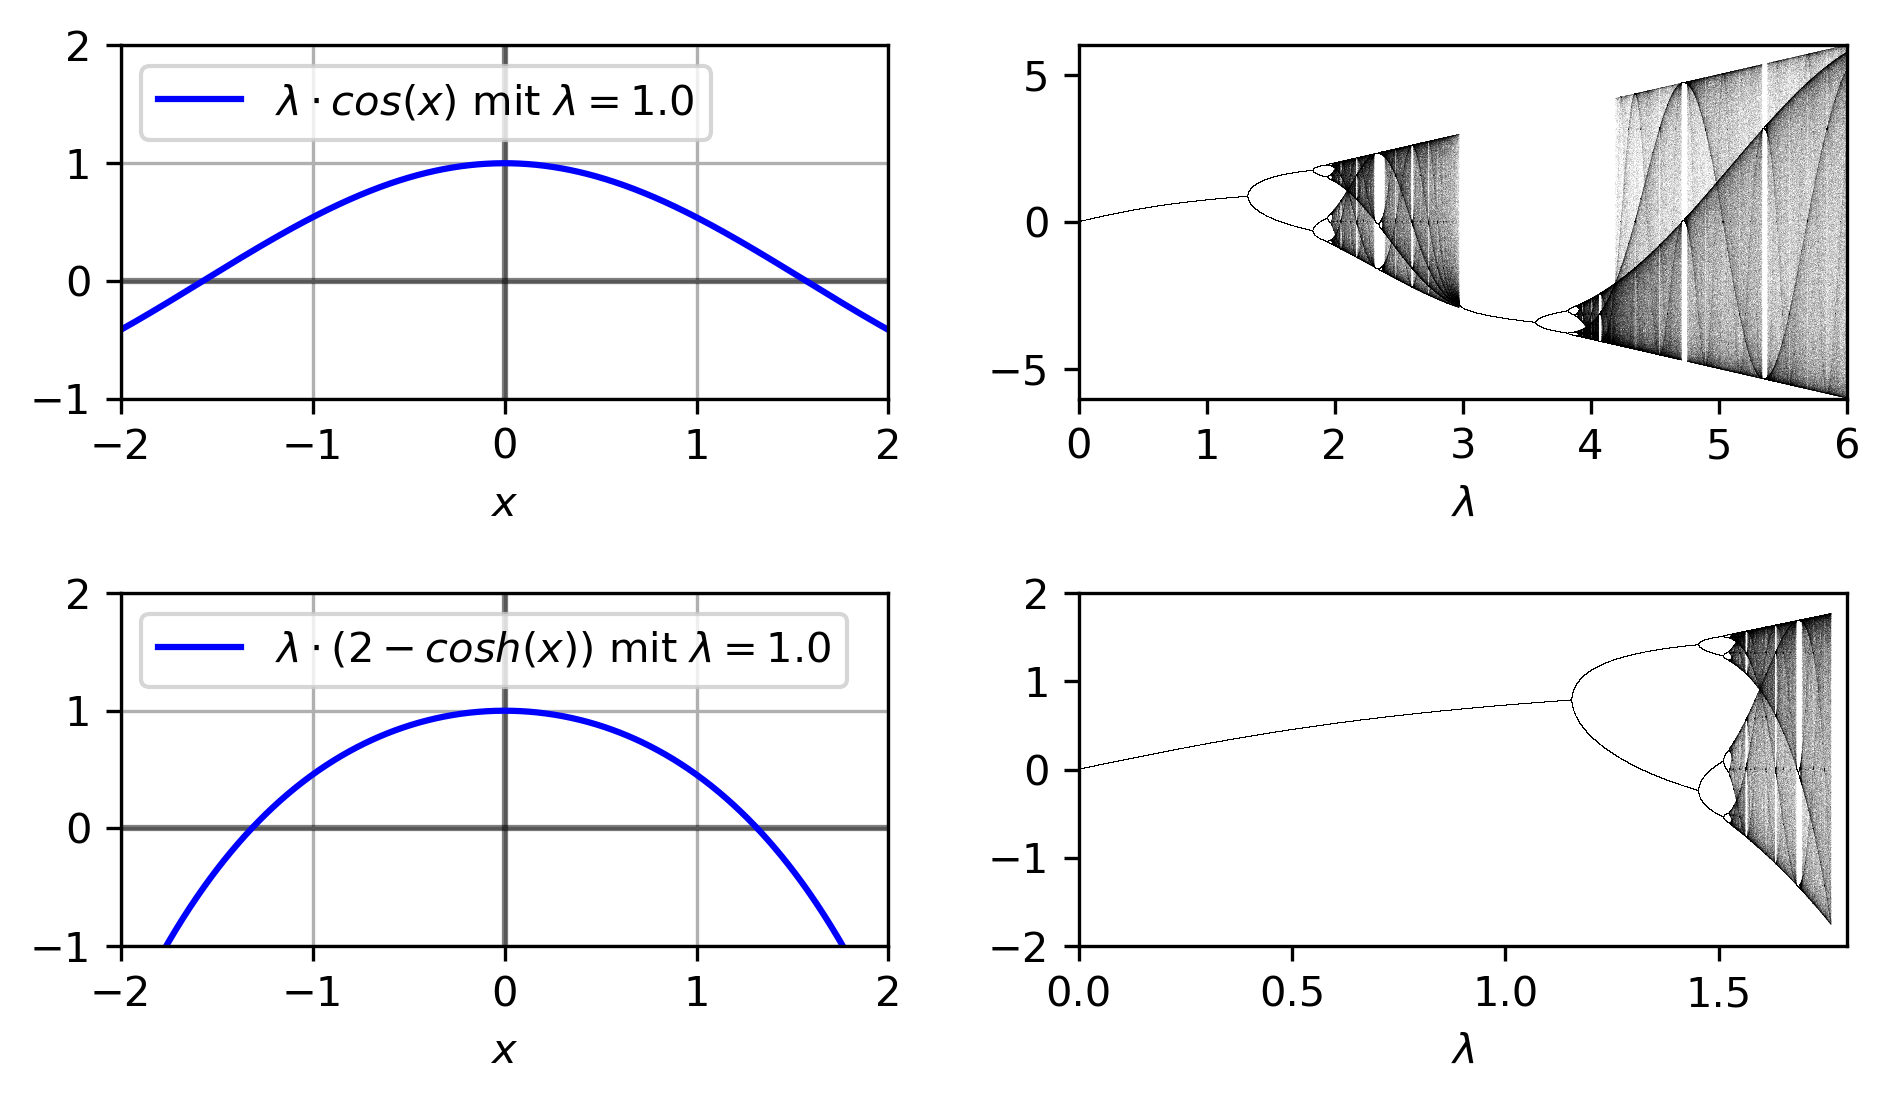
\includegraphics[width=\linewidth]{papers/logistic/figures/universal.png}
    \caption{
        Bifurkationsdiagramme von 
        $\lambda \cdot \cos(x)$
        und
        $\lambda \cdot (2 - \cosh(x))$.
        Links ist jeweils der Funktionsplot und
        rechts das dazugehörige Bifurkationsdiagramm. 
    }
    \label{fig:universal}
\end{figure}
\index{universelle Eigenschaft}%
Dieses Verhalten mit den Periodenverdoppelungen 
bis es schliesslich chaotisch wird und dann
immer wieder kurzen oszillierenden Fenstern im Chaos
ist keineswegs eine Eigenschaft, 
die nur die logistische Gleichung besitzt.
Man findet dieses Verhalten auch beim Iterieren 
von vielen anderen nichtlinearen Funktionen. 
Ein typisches Merkmal, 
an dem man Funktionen erkennt
die diese Eigenschaften aufweisen, 
sind ``Hügel'' im Funktionsplot.
Als Beispiel dazu sind in Abbildung \ref{fig:universal} links
die beiden Funktionen
$\lambda \cdot \cos(x)$
und
$\lambda \cdot (2 - \cosh(x))$
abgebildet.
Beide Funktionen haben, wie auch schon die Funktion
der logistischen Gleichung, einen Hügel. 
Rechts sind die Bifurkationsdiagramme dieser beiden
Funktionen abgebildet. 
Die Ähnlichkeiten zum Bifurkationsdiagramm der logistischen
Gleichung sind deutlich sichtbar. 
Besonders interessant wird es, wenn man
bei diesen Funktionen im Bifurkationsdiagramm 
die Periodenverdoppelungen genauer anschaut.
Denn wenn man das Verhältnis der Breite einer Periode
zur Breite der vorherigen Periode im Limit
anschaut, also 
$
    \lim_{n\to\infty}(\frac{\lambda_{n-1} - \lambda_{n-2}}{\lambda_n - \lambda_{n-1}})
$
wobei $\lambda_n$ der Wert von $\lambda$ bei der $n$-ten
Periodenverdoppelung ist,
dann kommt man auf die Zahl $\delta \approx 4.6692$.
Diese Zahl hat den Namen ``Feigenbaum-Konstante''.
Es ist irrelevant, welche Kaskade von Periodenverdoppelungen
\index{Kaskade von Periodenverdoppelungen}%
bei diesen Funktionen
gewählt wird, im Limit kommt schlussendlich immer diese Zahl heraus. 
Die Feigenbaum-Konstante findet man auf die genau gleiche Art 
\index{Feigenbaum-Konstante}%
auch in der logistischen Gleichung und in vielen anderen
Funktionen, die einen einzelnen ``Hügel'' haben, wieder.
Dadurch haben alle diese Funktionen durch die 
Feigenbaum-Konstante eine universale Eigenschaft.
Es ist überhaupt nicht offentsichtlich warum das so
sein sollte und es hat Mitchell Feigenbaum, 
\index{Feigenbaum, Mitchell}%
den Entdecker dieser Konstante, und andere Mathematiker 
viel Arbeit gekostet, diese Eigenschaft zu erforschen. 

Abschliessend können wir so aus diesen Erkenntnissen direkt 
noch etwas für die weitere Numerik mitnehmen.
Offenbar können sich Funktionen beim Iterieren sehr 
unerwartet verhalten. 
Gerade in der Numerik bauen viele Verfahren
auf iterativen Algorithmen auf. 
Deswegen schadet es sicherlich nicht,
wenn man sich bewusst ist, dass beim Iterieren von
scheinbar einfachen Funktionen so ein ``wildes'' 
Verhalten enstehen kann. 
